% shared preamble of the theory figures (white background, purple / black theme, sans-serif)
\documentclass[tikz,border=8pt]{standalone}
\usepackage[T1]{fontenc}
\usepackage[scaled=0.92]{helvet}
\renewcommand{\familydefault}{\sfdefault}
\usepackage{amsmath,amssymb}
\usepackage[helvet]{sfmath}
\usetikzlibrary{arrows.meta,calc,decorations.pathreplacing,positioning,backgrounds}
\definecolor{ink}{HTML}{1A1A1F}
\definecolor{cohesin}{HTML}{6A3DE8}
\definecolor{condensin}{HTML}{1BAF7A}
\definecolor{fwd}{HTML}{D1303F}      % CTCF pointing right
\definecolor{rev}{HTML}{2B62D9}      % CTCF pointing left
\definecolor{panel}{HTML}{F8F6FD}
\definecolor{panelline}{HTML}{E3DDF5}
\tikzset{
  fiber/.style={line width=2.1pt,ink,line cap=round,line join=round},
  halo/.style={line width=6pt,white,line cap=round},
  lab/.style={font=\small,text=ink},
  note/.style={font=\footnotesize,text=ink!60},
  hd/.style={font=\bfseries\small,text=ink,anchor=west},
  leader/.style={line width=0.6pt,ink!45},
}
% soft panel, numbered badge, heading
\newcommand{\panelbg}[4]{\draw[rounded corners=9pt,fill=panel,draw=panelline,line width=0.9pt] (#1,#2) rectangle (#3,#4);}
\newcommand{\badge}[3]{\fill[ink] (#1,#2) circle (0.21);\node[white,font=\bfseries\footnotesize] at (#1,#2) {#3};}
% CTCF: a protein on the fibre carrying an arrow that gives the motif direction (f = right, r = left)
\newcommand{\protf}[2]{\draw[rounded corners=3.5pt,line width=0.6pt,draw=fwd!65!black,fill=fwd] (#1-0.3,#2-0.19) rectangle (#1+0.3,#2+0.19);
  \draw[white,line width=1.5pt,-{Stealth[length=3.4pt,width=4.4pt]}] (#1-0.15,#2)--(#1+0.16,#2);}
\newcommand{\protr}[2]{\draw[rounded corners=3.5pt,line width=0.6pt,draw=rev!65!black,fill=rev] (#1-0.3,#2-0.19) rectangle (#1+0.3,#2+0.19);
  \draw[white,line width=1.5pt,-{Stealth[length=3.4pt,width=4.4pt]}] (#1+0.15,#2)--(#1-0.16,#2);}
\newcommand{\prot}[3]{\csname prot#3\endcsname{#1}{#2}}
% ring seen at an angle, drawn as a tube (dark outline, light core); back half and front half
\newcommand{\ringpart}[5]{\draw[line width=4.6pt,#3!80!black,line cap=round] ([shift={(#1,#2)}]#4:0.55 and 0.21) arc[start angle=#4,end angle=#5,x radius=0.55,y radius=0.21];
  \draw[line width=2.4pt,#3!55!white,line cap=round] ([shift={(#1,#2)}]#4:0.55 and 0.21) arc[start angle=#4,end angle=#5,x radius=0.55,y radius=0.21];}
\newcommand{\ringback}[3]{\ringpart{#1}{#2}{#3}{180}{0}}
\newcommand{\ringfront}[3]{\ringpart{#1}{#2}{#3}{180}{360}}
% smooth loop whose foot (ring) is at (cx,y0): half-width W, height H, ring colour
\newcommand{\lloop}[5]{%
  \ringback{#1}{#2}{#5}%
  \draw[fiber] (#1-0.3,#2) .. controls (#1-0.3,#2+0.25*#4) and (#1-#3,#2+0.2*#4) .. (#1-#3,#2+0.55*#4)
     .. controls (#1-#3,#2+0.95*#4) and (#1-0.5*#3,#2+#4) .. (#1,#2+#4)
     .. controls (#1+0.5*#3,#2+#4) and (#1+#3,#2+0.95*#4) .. (#1+#3,#2+0.55*#4)
     .. controls (#1+#3,#2+0.2*#4) and (#1+0.3,#2+0.25*#4) .. (#1+0.3,#2);%
  \ringfront{#1}{#2}{#5}}
% gently undulating fibre from x0 to the loop foot at cx (height y0), and from x1
\newcommand{\base}[4]{%
  \draw[fiber] plot[smooth] coordinates {(#1,0.05) (#1+0.35*#3-0.35*#1,-0.05) (#3-1.4,0.04)} .. controls (#3-0.6,0.02) and (#3-0.3,0.05) .. (#3-0.3,#4);
  \draw[fiber] plot[smooth] coordinates {(#2,-0.05) (#2-0.35*#2+0.35*#3,0.05) (#3+1.4,-0.04)} .. controls (#3+0.6,-0.02) and (#3+0.3,0.05) .. (#3+0.3,#4);}
% stop sign for a blocked leg and a leg arrow
\newcommand{\stopbar}[3]{\draw[#3,line width=2.4pt,line cap=round] (#1,#2-0.2)--(#1,#2+0.2);}
\newcommand{\legarrow}[3]{\draw[cohesin,line width=1.6pt,-{Stealth[length=5pt,width=6pt]},line cap=round] (#1,#3)--(#2,#3);}

\definecolor{A}{HTML}{D1303F}\definecolor{B}{HTML}{5B4FD6}
\tikzset{ln/.style={line width=0.7pt,ink!45},cur/.style={line width=1.8pt,cohesin},thin/.style={line width=0.9pt},
  mv/.style={line width=1.2pt,ink!70,-{Stealth[length=5pt,width=6pt]}},box/.style={rounded corners=5pt,draw=cohesin!70,fill=white,line width=0.9pt,align=center,font=\small,text=ink,inner sep=4pt}}
\begin{document}
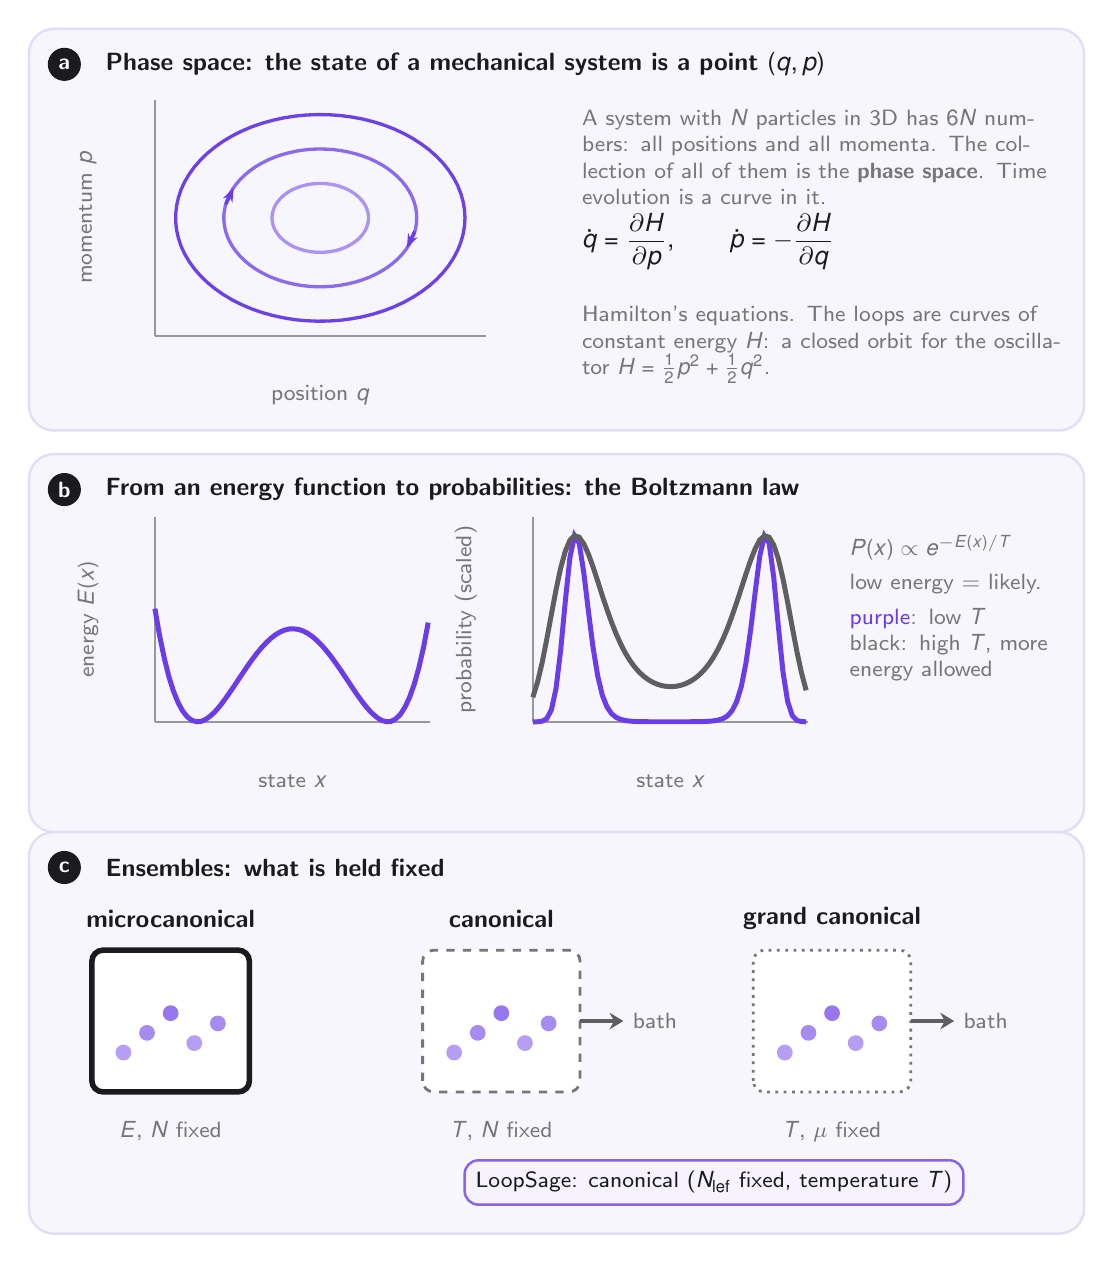
\begin{tikzpicture}
  \panelbg{0}{8.8}{13.4}{13.9}\badge{0.45}{13.450000000000001}{a}\node[hd] at (0.85,13.450000000000001) {Phase space: the state of a mechanical system is a point $(q,p)$};
  \panelbg{0}{3.7}{13.4}{8.5}\badge{0.45}{8.05}{b}\node[hd] at (0.85,8.05) {From an energy function to probabilities: the Boltzmann law};
  \panelbg{0}{-1.4}{13.4}{3.7}\badge{0.45}{3.25}{c}\node[hd] at (0.85,3.25) {Ensembles: what is held fixed};
  \draw[ln] (1.6,10.0)--(5.800000000000001,10.0);\draw[ln] (1.6,10.0)--(1.6,13.0);
  \node[note] at (3.70,9.25) {position $q$};
  \node[note,rotate=90] at (0.75,11.50) {momentum $p$};
  \draw[line width=1.2pt,cohesin!56] plot coordinates {(4.312,11.500) (4.311,11.535) (4.305,11.569) (4.295,11.603) (4.282,11.637) (4.265,11.669) (4.244,11.701) (4.220,11.731) (4.193,11.760) (4.162,11.787) (4.129,11.812) (4.093,11.836) (4.054,11.857) (4.013,11.876) (3.970,11.893) (3.926,11.907) (3.880,11.918) (3.833,11.927) (3.785,11.933) (3.737,11.937) (3.688,11.937) (3.639,11.935) (3.591,11.931) (3.543,11.923) (3.497,11.913) (3.452,11.900) (3.408,11.885) (3.366,11.867) (3.326,11.847) (3.289,11.824) (3.254,11.800) (3.222,11.774) (3.193,11.746) (3.168,11.716) (3.145,11.685) (3.126,11.653) (3.111,11.620) (3.100,11.586) (3.092,11.552) (3.088,11.517) (3.088,11.483) (3.092,11.448) (3.100,11.414) (3.111,11.380) (3.126,11.347) (3.145,11.315) (3.168,11.284) (3.193,11.254) (3.222,11.226) (3.254,11.200) (3.289,11.176) (3.326,11.153) (3.366,11.133) (3.408,11.115) (3.452,11.100) (3.497,11.087) (3.543,11.077) (3.591,11.069) (3.639,11.065) (3.688,11.063) (3.737,11.063) (3.785,11.067) (3.833,11.073) (3.880,11.082) (3.926,11.093) (3.970,11.107) (4.013,11.124) (4.054,11.143) (4.093,11.164) (4.129,11.188) (4.162,11.213) (4.193,11.240) (4.220,11.269) (4.244,11.299) (4.265,11.331) (4.282,11.363) (4.295,11.397) (4.305,11.431) (4.311,11.465) (4.312,11.500)};
  \draw[line width=1.2pt,cohesin!77] plot coordinates {(4.925,11.500) (4.921,11.570) (4.910,11.639) (4.890,11.707) (4.864,11.774) (4.829,11.839) (4.788,11.902) (4.740,11.962) (4.685,12.020) (4.624,12.074) (4.558,12.125) (4.485,12.172) (4.408,12.214) (4.327,12.252) (4.241,12.285) (4.152,12.313) (4.060,12.336) (3.966,12.354) (3.870,12.367) (3.773,12.373) (3.676,12.375) (3.578,12.371) (3.482,12.361) (3.387,12.346) (3.294,12.325) (3.203,12.300) (3.116,12.269) (3.032,12.234) (2.953,12.193) (2.878,12.149) (2.808,12.100) (2.744,12.047) (2.687,11.992) (2.635,11.932) (2.590,11.871) (2.553,11.807) (2.522,11.740) (2.499,11.673) (2.484,11.604) (2.476,11.535) (2.476,11.465) (2.484,11.396) (2.499,11.327) (2.522,11.260) (2.553,11.193) (2.590,11.129) (2.635,11.068) (2.687,11.008) (2.744,10.953) (2.808,10.900) (2.878,10.851) (2.953,10.807) (3.032,10.766) (3.116,10.731) (3.203,10.700) (3.294,10.675) (3.387,10.654) (3.482,10.639) (3.578,10.629) (3.676,10.625) (3.773,10.627) (3.870,10.633) (3.966,10.646) (4.060,10.664) (4.152,10.687) (4.241,10.715) (4.327,10.748) (4.408,10.786) (4.485,10.828) (4.558,10.875) (4.624,10.926) (4.685,10.980) (4.740,11.038) (4.788,11.098) (4.829,11.161) (4.864,11.226) (4.890,11.293) (4.910,11.361) (4.921,11.430) (4.925,11.500)};
  \draw[line width=1.2pt,cohesin!98] plot coordinates {(5.538,11.500) (5.532,11.604) (5.514,11.708) (5.485,11.810) (5.445,11.911) (5.394,12.008) (5.332,12.103) (5.260,12.194) (5.178,12.280) (5.087,12.361) (4.986,12.437) (4.878,12.507) (4.762,12.571) (4.640,12.628) (4.511,12.678) (4.378,12.720) (4.240,12.755) (4.099,12.781) (3.955,12.800) (3.810,12.810) (3.663,12.812) (3.518,12.806) (3.373,12.792) (3.230,12.769) (3.091,12.738) (2.955,12.700) (2.824,12.654) (2.698,12.600) (2.579,12.540) (2.467,12.473) (2.363,12.400) (2.267,12.321) (2.180,12.237) (2.103,12.149) (2.036,12.056) (1.979,11.960) (1.933,11.861) (1.899,11.759) (1.876,11.656) (1.864,11.552) (1.864,11.448) (1.876,11.344) (1.899,11.241) (1.933,11.139) (1.979,11.040) (2.036,10.944) (2.103,10.851) (2.180,10.763) (2.267,10.679) (2.363,10.600) (2.467,10.527) (2.579,10.460) (2.698,10.400) (2.824,10.346) (2.955,10.300) (3.091,10.262) (3.230,10.231) (3.373,10.208) (3.518,10.194) (3.663,10.188) (3.810,10.190) (3.955,10.200) (4.099,10.219) (4.240,10.245) (4.378,10.280) (4.511,10.322) (4.640,10.372) (4.762,10.429) (4.878,10.493) (4.986,10.563) (5.087,10.639) (5.178,10.720) (5.260,10.806) (5.332,10.897) (5.394,10.992) (5.445,11.089) (5.485,11.190) (5.514,11.292) (5.532,11.396) (5.538,11.500)};
  \draw[cohesin,line width=1.2pt,-{Stealth[length=5pt]}] (4.90,11.33)--(4.80,11.12);
  \draw[cohesin,line width=1.2pt,-{Stealth[length=5pt]}] (2.50,11.67)--(2.60,11.88);
  \node[note] at (3.70,10.00) {};
  \node[note,text width=6.2cm,anchor=north west] at (6.9,13.0) {A system with $N$ particles in 3D has $6N$ numbers: all positions and all momenta. The collection of all of them is the \textbf{phase space}. Time evolution is a curve in it.};
  \node[lab,anchor=west] at (6.9,11.2) {$\dot q=\dfrac{\partial H}{\partial p},\qquad \dot p=-\dfrac{\partial H}{\partial q}$};
  \node[note,text width=6.2cm,anchor=north west] at (6.9,10.5) {Hamilton's equations. The loops are curves of constant energy $H$: a closed orbit for the oscillator $H=\tfrac12p^2+\tfrac12q^2$.};
  \draw[ln] (1.6,5.1)--(5.1,5.1);\draw[ln] (1.6,5.1)--(1.6,7.699999999999999);
  \node[note] at (3.35,4.35) {state $x$};
  \node[note,rotate=90] at (0.75,6.40) {energy $E(x)$};
  \draw[cur] plot coordinates {(1.600,6.537) (1.659,6.197) (1.718,5.913) (1.776,5.679) (1.835,5.491) (1.894,5.345) (1.953,5.237) (2.012,5.162) (2.071,5.118) (2.129,5.101) (2.188,5.106) (2.247,5.132) (2.306,5.175) (2.365,5.231) (2.424,5.299) (2.482,5.376) (2.541,5.459) (2.600,5.545) (2.659,5.634) (2.718,5.722) (2.776,5.808) (2.835,5.891) (2.894,5.969) (2.953,6.040) (3.012,6.103) (3.071,6.159) (3.129,6.204) (3.188,6.240) (3.247,6.265) (3.306,6.279) (3.365,6.281) (3.424,6.273) (3.482,6.254) (3.541,6.223) (3.600,6.183) (3.659,6.132) (3.718,6.073) (3.776,6.005) (3.835,5.931) (3.894,5.850) (3.953,5.766) (4.012,5.678) (4.071,5.589) (4.129,5.502) (4.188,5.417) (4.247,5.337) (4.306,5.264) (4.365,5.202) (4.424,5.152) (4.482,5.117) (4.541,5.101) (4.600,5.106) (4.659,5.137) (4.718,5.195) (4.776,5.286) (4.835,5.413) (4.894,5.579) (4.953,5.790) (5.012,6.048) (5.071,6.360)};
  \draw[ln] (6.4,5.1)--(9.9,5.1);\draw[ln] (6.4,5.1)--(6.4,7.699999999999999);
  \node[note] at (8.15,4.35) {state $x$};
  \node[note,rotate=90] at (5.55,6.40) {probability (scaled)};
  \draw[line width=1.8pt,cohesin] plot coordinates {(6.400,5.100) (6.459,5.101) (6.518,5.108) (6.576,5.140) (6.635,5.251) (6.694,5.522) (6.753,6.006) (6.812,6.631) (6.871,7.189) (6.929,7.464) (6.988,7.370) (7.047,6.993) (7.106,6.501) (7.165,6.040) (7.224,5.682) (7.282,5.439) (7.341,5.289) (7.400,5.203) (7.459,5.155) (7.518,5.130) (7.576,5.116) (7.635,5.109) (7.694,5.105) (7.753,5.103) (7.812,5.102) (7.871,5.101) (7.929,5.101) (7.988,5.101) (8.047,5.101) (8.106,5.101) (8.165,5.101) (8.224,5.101) (8.282,5.101) (8.341,5.101) (8.400,5.101) (8.459,5.102) (8.518,5.102) (8.576,5.104) (8.635,5.107) (8.694,5.112) (8.753,5.122) (8.812,5.140) (8.871,5.175) (8.929,5.240) (8.988,5.355) (9.047,5.547) (9.106,5.846) (9.165,6.260) (9.224,6.751) (9.282,7.207) (9.341,7.461) (9.400,7.372) (9.459,6.934) (9.518,6.311) (9.576,5.738) (9.635,5.361) (9.694,5.181) (9.753,5.118) (9.812,5.103) (9.871,5.100)};
  \draw[line width=1.8pt,ink!70] plot coordinates {(6.400,5.412) (6.459,5.603) (6.518,5.852) (6.576,6.146) (6.635,6.463) (6.694,6.775) (6.753,7.051) (6.812,7.267) (6.871,7.406) (6.929,7.464) (6.988,7.445) (7.047,7.361) (7.106,7.229) (7.165,7.065) (7.224,6.886) (7.282,6.703) (7.341,6.527) (7.400,6.363) (7.459,6.214) (7.518,6.084) (7.576,5.971) (7.635,5.875) (7.694,5.795) (7.753,5.729) (7.812,5.675) (7.871,5.632) (7.929,5.599) (7.988,5.574) (8.047,5.558) (8.106,5.549) (8.165,5.547) (8.224,5.552) (8.282,5.565) (8.341,5.585) (8.400,5.614) (8.459,5.652) (8.518,5.700) (8.576,5.760) (8.635,5.833) (8.694,5.921) (8.753,6.025) (8.812,6.147) (8.871,6.286) (8.929,6.443) (8.988,6.614) (9.047,6.794) (9.106,6.977) (9.165,7.150) (9.224,7.300) (9.282,7.410) (9.341,7.463) (9.400,7.445) (9.459,7.347) (9.518,7.168) (9.576,6.919) (9.635,6.622) (9.694,6.303) (9.753,5.994) (9.812,5.721) (9.871,5.500)};
  \node[note,text width=2.8cm,anchor=north west] at (10.3,7.6) {$P(x)\propto e^{-E(x)/T}$\\[3pt]low energy = likely.\\[3pt]\textcolor{cohesin}{purple}: low $T$\\black: high $T$, more energy allowed};
  \draw[rounded corners=4pt,ink,line width=2pt,fill=white] (0.8,0.4) rectangle (2.8,2.2);
  \fill[cohesin!50] (1.20,0.90) circle (0.1);
  \fill[cohesin!60] (1.50,1.15) circle (0.1);
  \fill[cohesin!70] (1.80,1.40) circle (0.1);
  \fill[cohesin!50] (2.10,1.02) circle (0.1);
  \fill[cohesin!60] (2.40,1.27) circle (0.1);
  \node[lab] at (1.8,2.6) {\bfseries microcanonical};\node[note] at (1.8,-0.1) {$E,\,N$ fixed};
  \draw[rounded corners=4pt,ink!60,line width=1pt,dashed,fill=white] (5.0,0.4) rectangle (7.0,2.2);
  \fill[cohesin!50] (5.40,0.90) circle (0.1);
  \fill[cohesin!60] (5.70,1.15) circle (0.1);
  \fill[cohesin!70] (6.00,1.40) circle (0.1);
  \fill[cohesin!50] (6.30,1.02) circle (0.1);
  \fill[cohesin!60] (6.60,1.27) circle (0.1);
  \draw[mv] (7.0,1.3)--(7.55,1.3);\node[note] at (7.95,1.3) {bath};
  \node[lab] at (6.0,2.6) {\bfseries canonical};\node[note] at (6.0,-0.1) {$T,\,N$ fixed};
  \draw[rounded corners=4pt,ink!60,line width=1pt,dotted,fill=white] (9.200000000000001,0.4) rectangle (11.200000000000001,2.2);
  \fill[cohesin!50] (9.60,0.90) circle (0.1);
  \fill[cohesin!60] (9.90,1.15) circle (0.1);
  \fill[cohesin!70] (10.20,1.40) circle (0.1);
  \fill[cohesin!50] (10.50,1.02) circle (0.1);
  \fill[cohesin!60] (10.80,1.27) circle (0.1);
  \draw[mv] (11.200000000000001,1.3)--(11.75,1.3);\node[note] at (12.150000000000002,1.3) {bath};
  \node[lab] at (10.200000000000001,2.6) {\bfseries grand canonical};\node[note] at (10.200000000000001,-0.1) {$T,\,\mu$ fixed};
  \node[box,draw=cohesin!80,fill=cohesin!6,font=\footnotesize] at (8.7,-0.75) {LoopSage: canonical ($N_{\mathrm{lef}}$ fixed, temperature $T$)};
\end{tikzpicture}
\end{document}
